\documentclass[hyperref={pdfpagelabels=false}]{beamer}
\usepackage{lmodern}
\usepackage{graphicx}%este pacote é para figuras
\usepackage[utf8]{inputenc}
\usepackage[brazil]{babel}% este é para o texto
\usepackage[all]{xy}
\usepackage{tikz} % Pacote para gráficos

%\usepackege{multirow,colortbl,array} % estes pacotes são para fazer múltiplas linhas, colorir as celulas e formatar a tabela.

\usepackage{subfig} % este é para fazer sub figuras

\usetheme{Copenhagen}

\title{Mineração de Dados Distribuída Aplicada à Detecção de Desvios Comportamentais no Contexto da Internet das Coisas}  

\author{Ricardo de Azevedo Brand\~{a}o \\ Orientador: Ronaldo Ribeiro Goldschmidt}

\institute {Mestrando em Sistemas e Computação \\ Instituto Militar de Engenharia }

\begin{document}
\begin{frame}
\titlepage
\end{frame} 

\begin{frame}
	\frametitle{Tópicos abordados}
	\footnotesize{\tableofcontents}
\end{frame} 

\section{Introdução}

\subsection{Contextualiza\c{c}\~{a}o}

\begin{frame}
	\frametitle{Introdução}
	\begin{figure}[h]
		\centering
		\includegraphics[scale=0.45]{img/IoT.png}
		\caption{\scriptsize{Internet das coisas (Fonte: Creative Commons).}}
		\label{fig:IoT}
	\end{figure}	

\end{frame}

\begin{frame}
	\frametitle{Motivação}

	\begin{itemize}
    	\item Internet das coisas
	        \begin{itemize}
    	    	\item Coisas (sensores e atuadores) conectadas
       		   	\item Internet (Identificadas por IP)
          		\item Dados Gerados
                	\begin{itemize}
                    	\item Sobre as coisas
                        \item Interação Humanos x Humanos
                        \item Interação Humanos x Coisas
                        \item Interação Coisas x Coisas
                    \end{itemize}
        	\end{itemize}
	\end{itemize}		
\end{frame}

\begin{frame}
	\frametitle{Motivação}
    
	\begin{itemize}
		\item Crescimento expondencial de coisas conectadas
		    \begin{figure}
 		   		\centering
	        	\includegraphics[scale=0.3]{img/ransomwareIoT.jpeg}
  		    	\caption{\scriptsize{Fonte: Joy of Tech http://www.geekculture.com/joyoftech/joyarchives/2340.html}}
   			\end{figure}
	\end{itemize}   
\end{frame}

\subsection{Problema}
 
\begin{frame}

	\frametitle{Problema}	

	\begin{itemize}
    	\item Exemplos de Desafios \cite{000-000} \begin{itemize} 
        	\item Centralização na análise de dados  \begin{itemize}
      	    	\item Aumento no tráfego da rede
			\end{itemize}
       		\item Topologia Dinâmica \begin{itemize}
          		\item Nós aparecem e desaparecem
               	\item Mudanças constantes no tempo e espaço
			\end{itemize}
        	\item Identificação de comportamentos de Humanos e Coisas oo \begin{itemize}
        		\item Detecção de Desvios de Comportamentos
        	\end{itemize}
            % Em IV Discussions B - Potential use of IoTs
            % Também em III - Data Mining for IoT D - Frequent Pattern Mining 
        	\end{itemize}
	\end{itemize}
    
\end{frame}
 
\begin{frame}
	\frametitle{Problema}
    
    Trabalhos com Análise centralizada
    \linebreak
    \begin{itemize}
	    \item Sistema de Detecção de Intrusão \cite{004-000}
        \item Análise de padrões em apartamento inteligente \cite{009-038}
        \item Detecção de Falsos-positivos em leituras de Tags RFID \cite{000-015}
        \item Análise de Comportamento de Compras em Supermercados \cite{000-123}
        
    \end{itemize}
\end{frame} 
 
\subsection{Hipótese}
 
\begin{frame}
	\frametitle{Hipótese}
	
    \begin{itemize}
    	\item O uso de t\'{e}cnicas de minera\c{c}\~{a}o de dados distribu\'{i}da no cenário da Internet das Coisas pode contribuir para reduzir o tráfego de informações necessárias às análises de desvios de padrões de comportamento sem diminuir a qualidade dos padrões que seriam identificados por meio de técnicas de mineração de dados centralizada.
    \end{itemize}
\end{frame}

\subsection{Objetivo}
 
\begin{frame}
	\frametitle{Objetivo}

	\begin{itemize}
		\item Demonstrar que o uso de t\'{e}cnicas de minera\c{c}\~{a}o de dados distrubu\'{i}da no cenário da Internet das Coisas pode contribuir para reduzir o tráfego de informações necessárias às análises de desvios de padrões de comportamento sem diminuir a qualidade dos padrões que seriam identificados por meio de técnicas de mineração de dados centralizada.
	\end{itemize}

\end{frame}

\subsection{Método}  

\begin{frame}
	\frametitle{Método}
     \begin{itemize}
        	\item Revisão da Literatura
            \item Aprofundamento dos conceitos básicos \begin{itemize}
	            \item Internet das Coisas
  	         	\item Mineração de dados
            	\item (i) Clusterização
            	\item (ii) Sumarização de dados
            	\item (iii) Detecção de desvios
            	\item (iv) Mineracao de dados distribuída
            \end{itemize}
            \item Detalhamento da solução proposta \begin{itemize}
            	\item Mineração Distribuída
            	\item Sumarização de Modelos
            	\item Integração dos modelos sumarizados
            \end{itemize}
		\end{itemize}

\end{frame}

\begin{frame}
	\frametitle{Método}
     \begin{itemize}
            \item Implementação do protótipo
            \item Execução dos estudos de caso -- Análise de datasets:\begin{itemize}
            	\item Pulseira
            	\item Telemetria (carro / onibus)
            	\item Dados de clima
            \end{itemize}
%            \item Preparação dos datasets
%            \item Implementação dos algoritmos
%            \item Realização dos experimentos
%            \item Avaliação dos resultados
		\end{itemize}

\end{frame}

\subsection{Contribuições Esperadas}  

\begin{frame}
	\frametitle{Contribuições Esperadas}
	\begin{itemize}
		\item Maior eficiência na detecção de desvios de comportamento a partir de dados gerados por dispositivos de Internet das Coisas
        \item Abordagem que permita a redução no tráfego de dados necessários para análise em redes de dispositivos sem perda da qualidade da mineração dos dados 
        \item Modelo comparativo de trabalhos relacionados
        \item Ferramenta desenvolvida 
	\end{itemize}
\end{frame}
   
\section{Conceitos Básicos}

\begin{frame}
	%\frametitle{Conceitos Básicos}
    
    \Large{Internet Das Coisas} \\
    
    \normalsize{De acordo com \cite{000-004}} é a tecnologia que permitiu a mudança da Internet que conecta dispositivos de usuários finais para uma Internet usada para interconectar objetos físicos que se comunicam entre si e/ou com seres humanos para prover um determinado serviço.
    \begin{itemize}
	    \item \normalsize{Conceito construído em três pilares:} \begin{itemize}
		    \item Deve ser identificável
            \item Deve comunicar-se
            \item Deve Interagir
		    \end{itemize}
        
    \end{itemize}

\end{frame}

\begin{frame}

	%\frametitle{Conceitos Básicos}
    
    \Large{Mineração de Dados -- Clusterização}
    
    \begin{figure}
		\centering
	    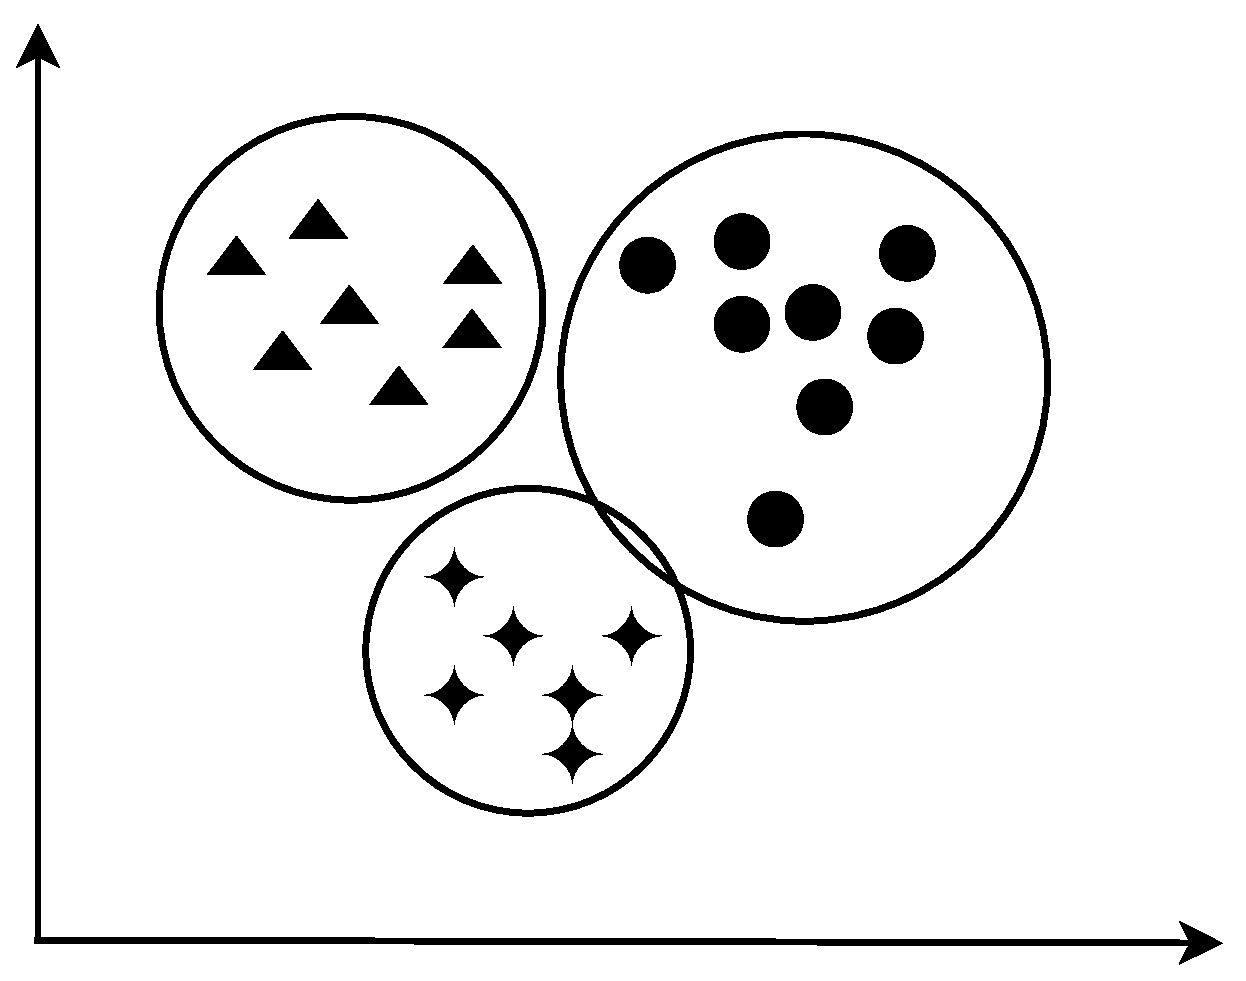
\includegraphics[scale=0.3]{img/Clustering.eps}
        \caption{\scriptsize{Clusterização}}
	\end{figure}
    

\end{frame}

\begin{frame}

	%\frametitle{Conceitos Básicos}
    
    \Large{Mineração de Dados - Clusterização}\linebreak
    \normalsize
   
    É a tarefa usada para separar os registros de um conjunto de dados em subconjutnos ou grupos (clusters) de tal forma que compartilhem um conjunto de propriedades comuns que os distingam dos elementos de outros clusters. \cite{goldschmidt2015data}
    \begin{itemize}
    \item \large{\textbf{Objetivo}} \\
    	\normalsize\textbf{Maximizar} a similaridade Intracluster e \textbf{Minimizar} a similaridade Intercluster
  		
    \end{itemize}
    

\end{frame}

\begin{frame}
	%\frametitle{Conceitos Básicos}
    
    	\Large{Mineração de Dados -- Sumarização}
        \begin{figure}
		\centering
	    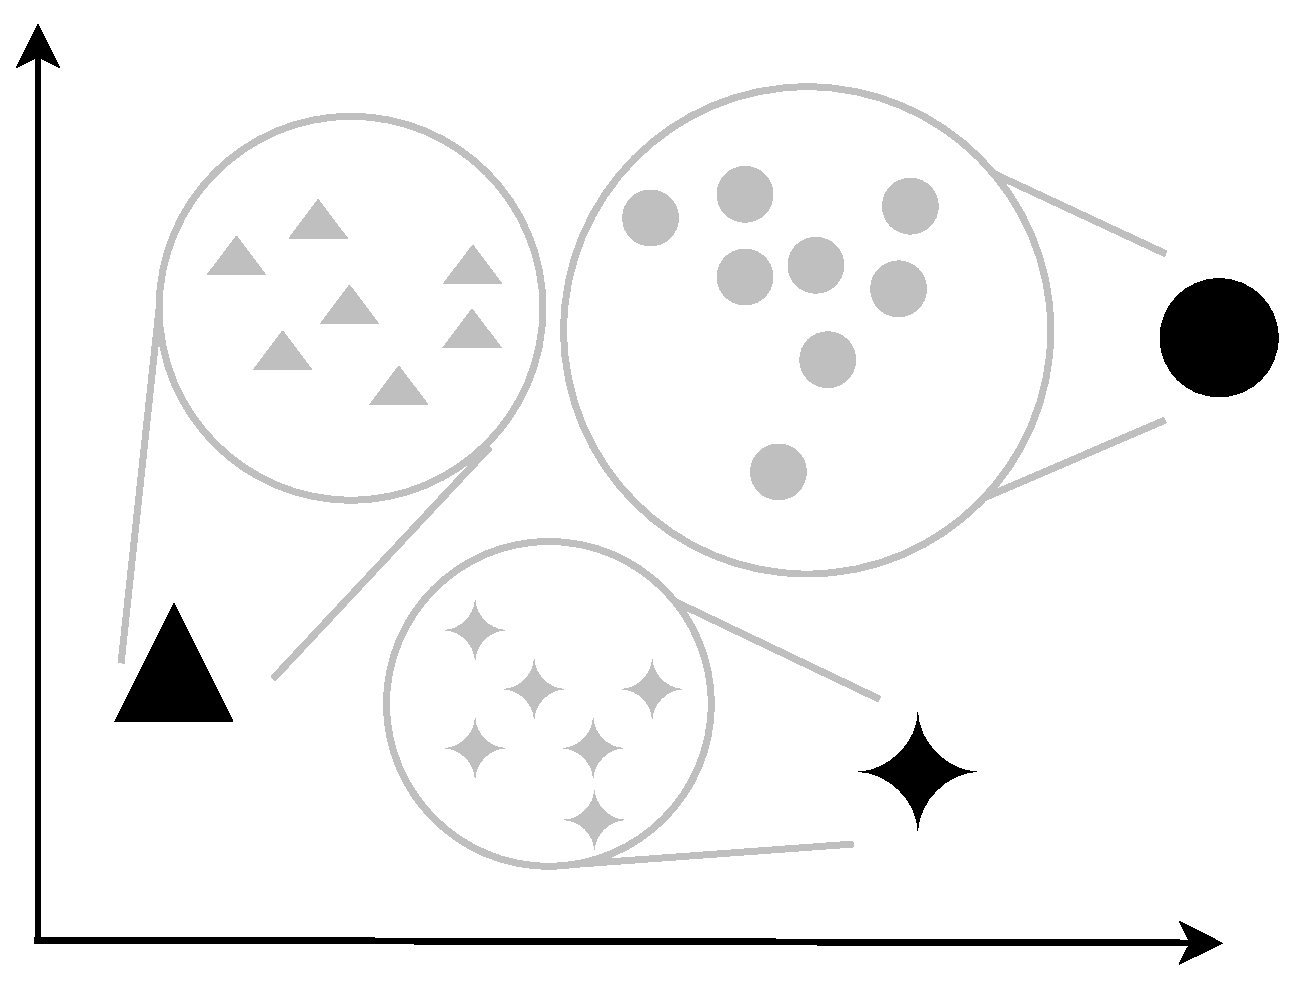
\includegraphics[scale=0.3]{img/Summarization.eps}
        \caption{\scriptsize{Sumarização}}
		\end{figure}
    

\end{frame}

\begin{frame}

	%\frametitle{Conceitos Básicos}
    
    \Large{Mineração de Dados -- Sumarização}\linebreak
    \normalsize
   
    De acordo com \cite{goldschmidt2015data}, é a tarefa usada para identificar e apresentar, de forma concisa e compreensível, as principais características de um conjunto de dados.
    \linebreak\linebreak Também conhecida como \textbf{Descrição de Conceitos}

\end{frame}

\begin{frame}
	%\frametitle{Conceitos Básicos}
    
    \Large{Mineração de Dados -- Detecção de Desvios}
    
        \begin{figure}
		\centering
	    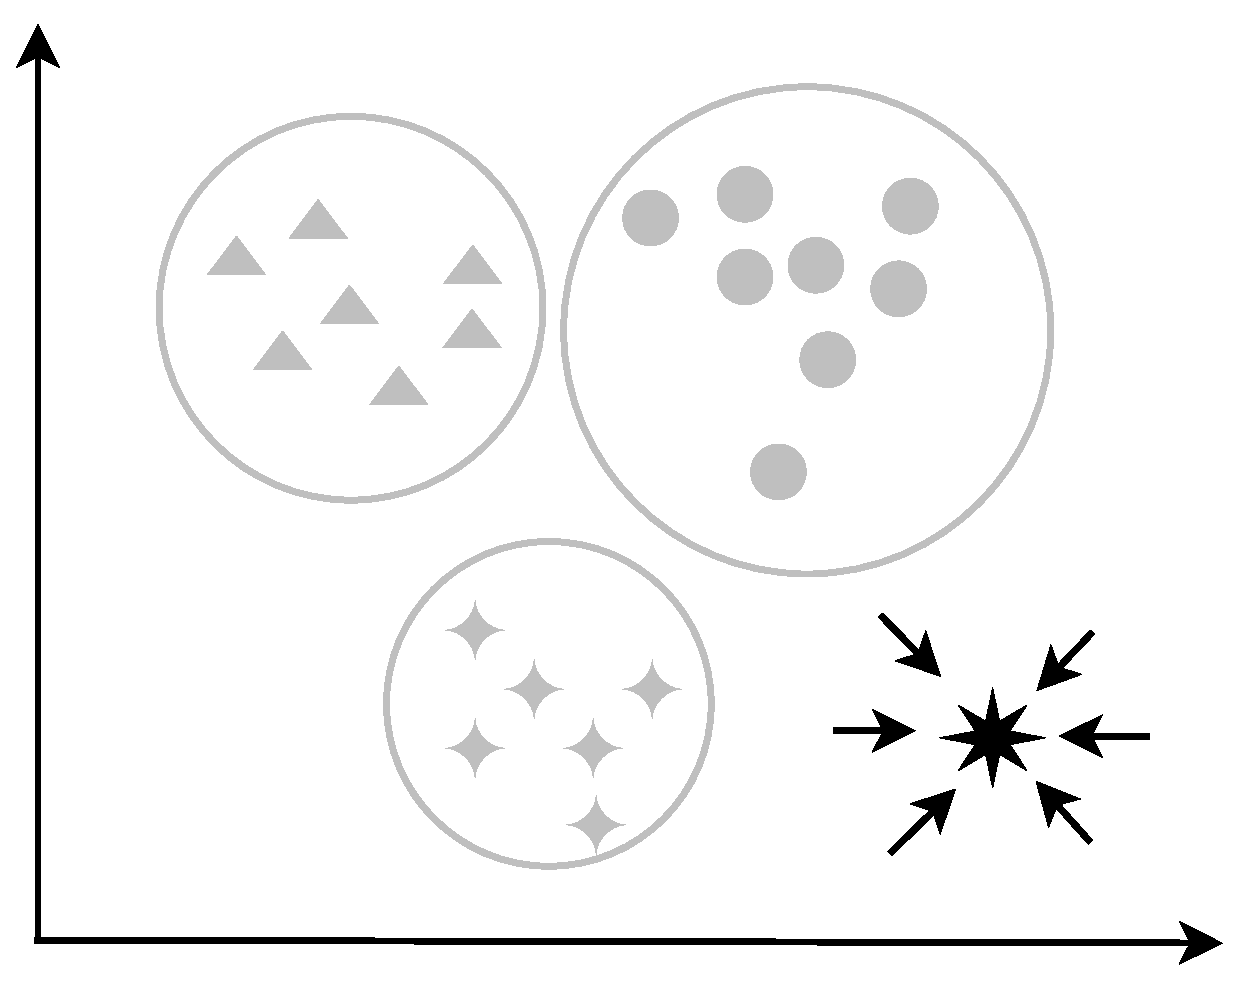
\includegraphics[scale=0.3]{img/Outlier.eps}
        \caption{\scriptsize{Detecção de Desvios}}
		\end{figure}

\end{frame}

\begin{frame}

	%\frametitle{Conceitos Básicos}
    
    \Large{Mineração de Dados -- Detecção de Desvios}\linebreak
    \normalsize
   
    Tem como objetivo identificar mudanças em padrões anteriormente percebidos. \cite{goldschmidt2015data}
    \linebreak\linebreak Identifica valores espúrios também conhecidos como \textit{outliers}

\end{frame}

\begin{frame}
	%\frametitle{Conceitos Básicos}
    
    \Large{Mineração de Dados -- Centralizada x Distribuída}
    \begin{figure}
     \subfloat[\scriptsize Mineração Centralizada]{%
       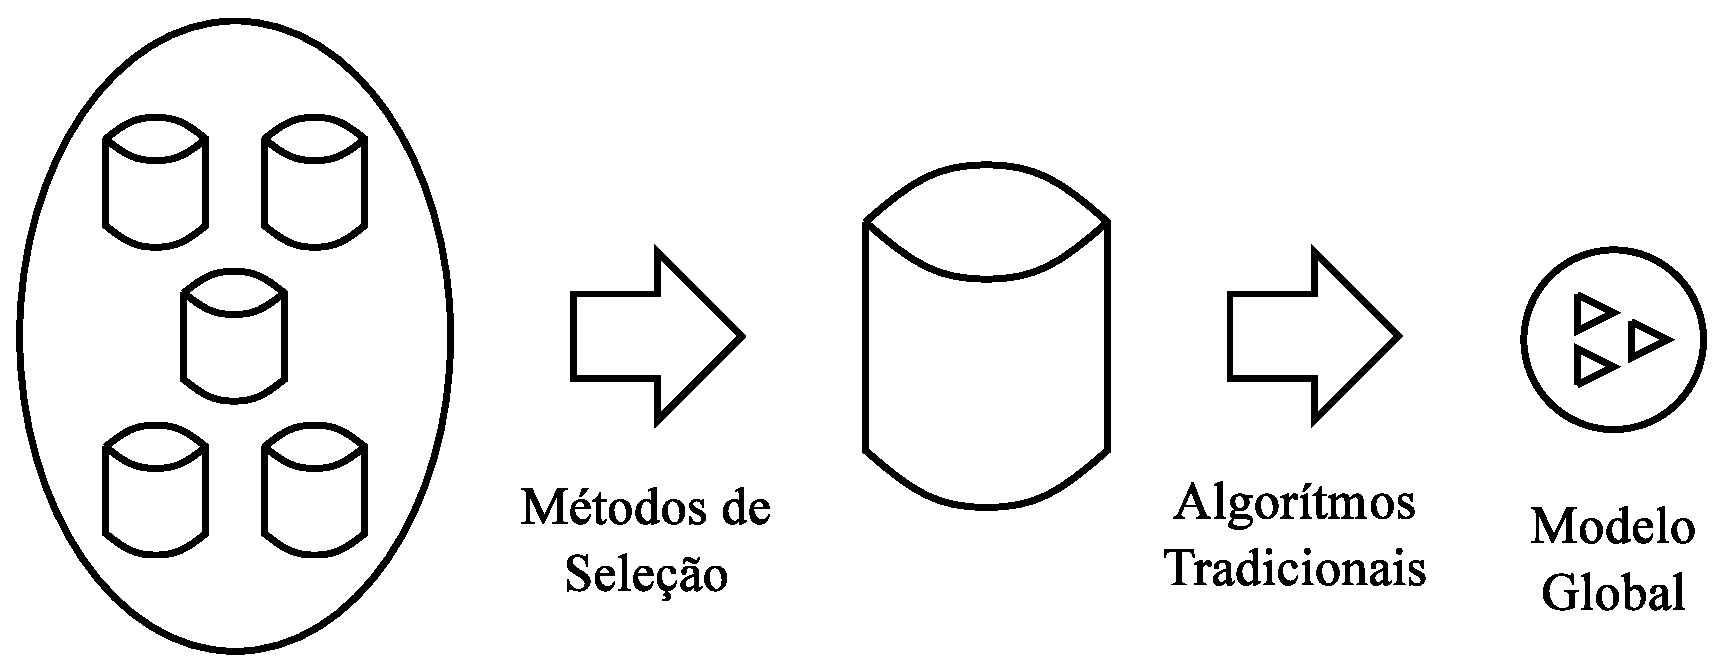
\includegraphics[width=0.45\textwidth]{img/MineracaoCentralizada.eps}
     }
     \hfill
     \subfloat[\scriptsize Mineração Distribuída]{%
       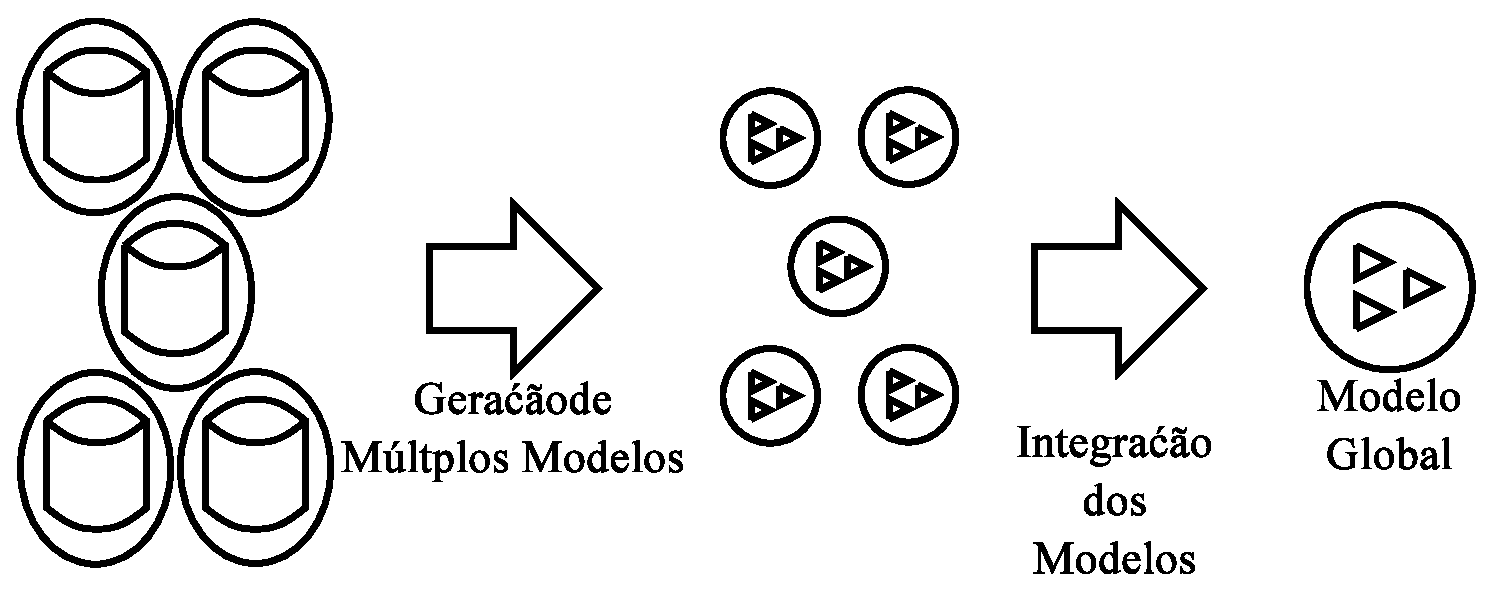
\includegraphics[width=0.45\textwidth]{img/MineracaoDistribuida.eps}
     }
     \caption{Mineração de Dados}
     \end{figure}
     
\end{frame}

\begin{frame}

	%\frametitle{Conceitos Básicos}
    
    \Large{Mineração de Dados -- Mineração de Dados Distribuída}\linebreak
    \normalsize
   
    Costuma ser ser utilizada em sistemas fracamente acoplados. \cite{goldschmidt2015data}
	\linebreak \linebreak Pode ser também utilizada nos seguintes casos: \cite{016-000} \begin{itemize}
    	\item Recursos computacionais geograficamente distribuídos
        \item Questões de privacidade ou dados sensiveis em ambiente distribuído
    \end{itemize}
\end{frame}

\section {Trabalhos relacionados}

\begin{frame}
	\frametitle{Trabalhos relacionados}

% Colocar os trabalhos citados no survey relacionados com o trabalho
% Verificar o que tem de análise de comportamento (em geral e os específicos em IoT)
% Verificar o que tem de análise distribuída (idem)

    Em \cite{000-000} é apresentado um survey sobre Mineração de dados para Internet das Coisas. (Qualis A1) \\
    Apresenta os desafios agrupados por:
	\begin{itemize}
		\item Infraestrutura
        \item Dados
        \item Algoritmos
        \item Segurança/Privacidade
	\end{itemize}

\end{frame}

\begin{frame}
	\frametitle{Trabalhos Relacionados}

	Em \cite{000-014} (Qualis A1) são abordados os desafios na mineração distribuída em redes de sensores sem fios -- WSN (Wireless Sensor Networks).
    Tem como foco analisar o trade-off entre:\begin{itemize}
	    \item Mineração centralizada com alto consumo de rede para transferência de dados
        \item Mineração nos sensores com limitações: \begin{itemize}
        \item Capacidade de processamento
        \item Consumo de energia
        \item Tempo de vida das baterias
        \end{itemize}
    \end{itemize}
    
\end{frame}

\begin{frame}
	\frametitle{Trabalhos Relacionados}
	
    \cite{001-000} (Qualis A1) apresenta um algorítimo genérico de Clusterização Descentralizada, o GDCluster.
    \linebreak 
    \linebreak
    A proposta é que cada nó faça uma sumarização dos seus dados para compartilhar entre os demais nós.
    \linebreak \linebreak
    O resultado é atingido analisando os dados internos com os dados sumarizados recebidos dos demais nós.
    \linebreak \linebreak
    O algoritmo considera o dinamismo dos dados, atribuindo uma idade a cada item do dataset.
    
\end{frame}

\begin{frame}
	\frametitle{Trabalhos Relacionados}
    Em \cite{017-000} é apresentado o algorítmo $D^{2}CA$ (Distributed Dynamic Clustering Algorithm) que explora a clusterização em plataforma distribuída, \textbf{maximizando} o paralelismo e \textbf{minimizando} a comunicação. 
    \begin{itemize}
	    \item Modelos locais gerados por clusterização (K-means)
        \item Cálculo dos contornos (usados como representantes dos clusters)
        \item Troca dos contornos entre nós vizinhos \begin{itemize}
	        \item Verificação de sobreposição de contornos
        \end{itemize}
        \item Fusão dos contornos em grupos
        \item Escolha de um líder entre os nós
        \item Processo repete-se até o nó central
    \end{itemize}

\end{frame}

\begin{frame}
	\frametitle{Trabalhos Relacionados - Algoritmo $D^{2}CA$}
    
    \begin{figure}
    
    \subfloat[\scriptsize Dataset 1]{%
       \includegraphics[width=0.35\textwidth]{img/D2CA-Dataset1.png}
     }
     \hfill
     \subfloat[\scriptsize Dataset 2]{%
       \includegraphics[width=0.4\textwidth]{img/D2CA-Dataset2.png}
     }
     \hfill
     \subfloat[\scriptsize Dataset 3]{%
       \includegraphics[width=0.4\textwidth]{img/D2CA-Dataset3.png}
     }

     \caption{Comparação Algoritmos \cite{017-000}}
     \end{figure}
     
\end{frame}

% Frame retirado -- Verificar o uso desse artigo. Talvez seja desnecessário

%\begin{frame}
%	\frametitle{Trabalhos Relacionados}
%    
%    Em \cite{000-062} (Qualis A1) é proposta uma abordagem no monitoramento e detecção de atividades diárias em uma casa inteligente.
%    \linebreak \linebreak
%    No lugar de utlizar aprendizagem supervisionada, é proposta uma abordagem automatizada para monitorar as atividades comuns e posterior detecção de mudanças no comportamento.
%\end{frame}

\begin{frame}

        \frametitle{Trabalhos Relacionados}
        
       Detecção de desivos de comportamento \begin{itemize}
               \item \cite{022-000} propõe uma nova formulação na detecção de \textit{outliers} com base na distância utilizando um algoritmo baseado em partições
               \item \cite{023-000} utiliza o algoritmo LOF (\it{Local Outlier Factor}) aplicado em um grid com o objetivo de reduzir o tempo de computação na descoberta de desvio de comportamentos.
       \end {itemize}
\end{frame}

\section{Solução Proposta}

\subsection{Visão Geral}  

\begin{frame}
	\frametitle{Visão Geral - Algoritmos de Clusterização}
    Análise dos Algorítmos para Mineração distribuída
   
	\begin{itemize}
	    \item GDCluster \cite{001-000}
        \item $D^{2}CA$ \cite{017-000} 
    \end{itemize}
    
    Geração dos modelos individuais e de grupo \begin{itemize}
            \item Utilização da abordagem dos algoritmos estudados
            \item Adequação dos algoritmos ao contexto da internet das coisas \begin{itemize}
                    \item Poucos recursos computacionais
                    \item Redução no tráfego de informações
            \end{itemize}
    \end{itemize}
%       
\end{frame}
%
\begin{frame}
	\frametitle{Visão Geral -- Módulos Distribuídos}
    \begin{figure}
		\centering
	    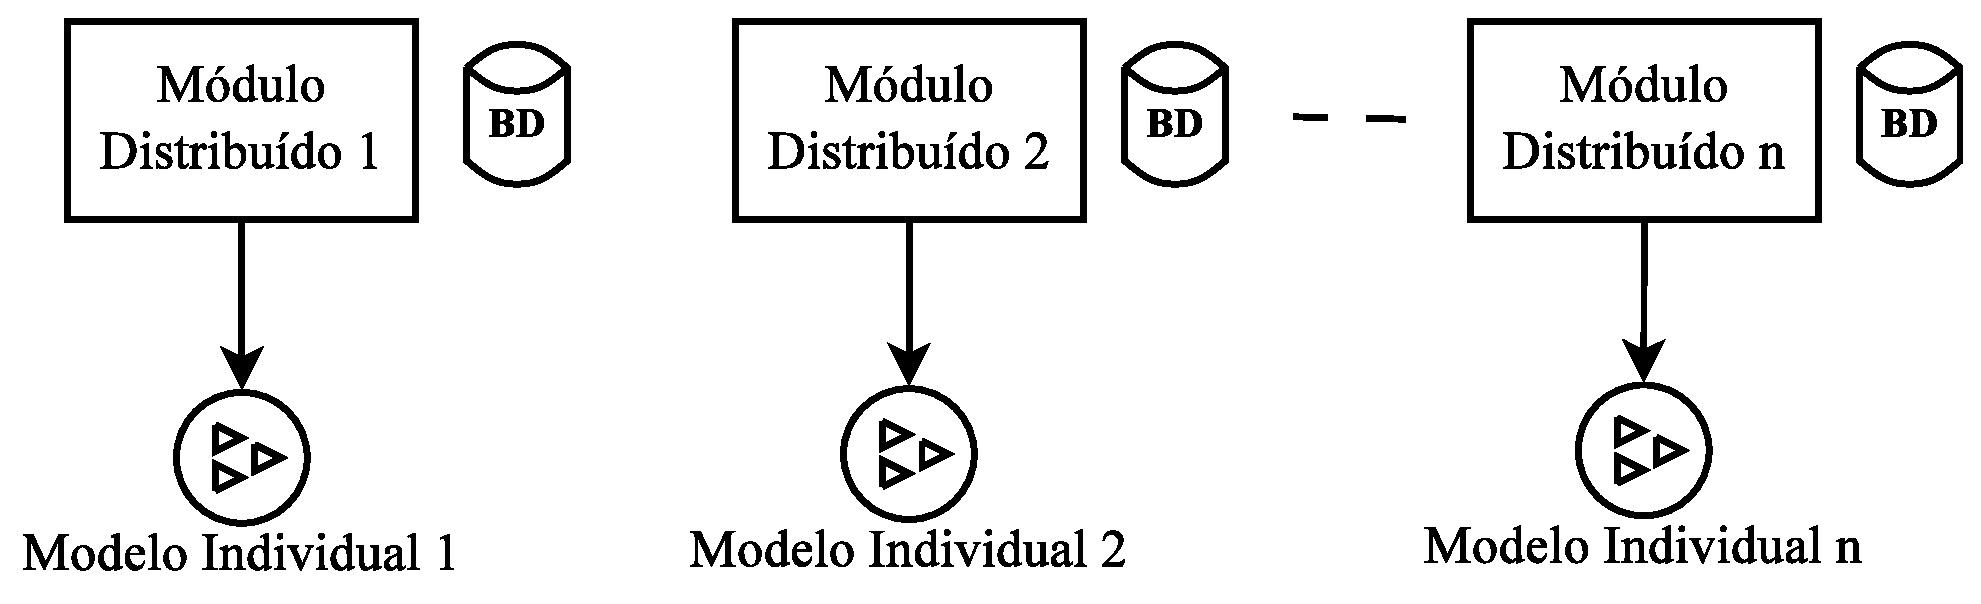
\includegraphics[scale=0.35]{img/VisaoGeral-00}
  		\caption{\scriptsize{Geração de Modelos Individuais}}
   	\end{figure}
%
\end{frame}
%
\begin{frame}
	\frametitle{Visão Geral -- Módulos Distribuídos}
    \begin{figure}
		\centering
	    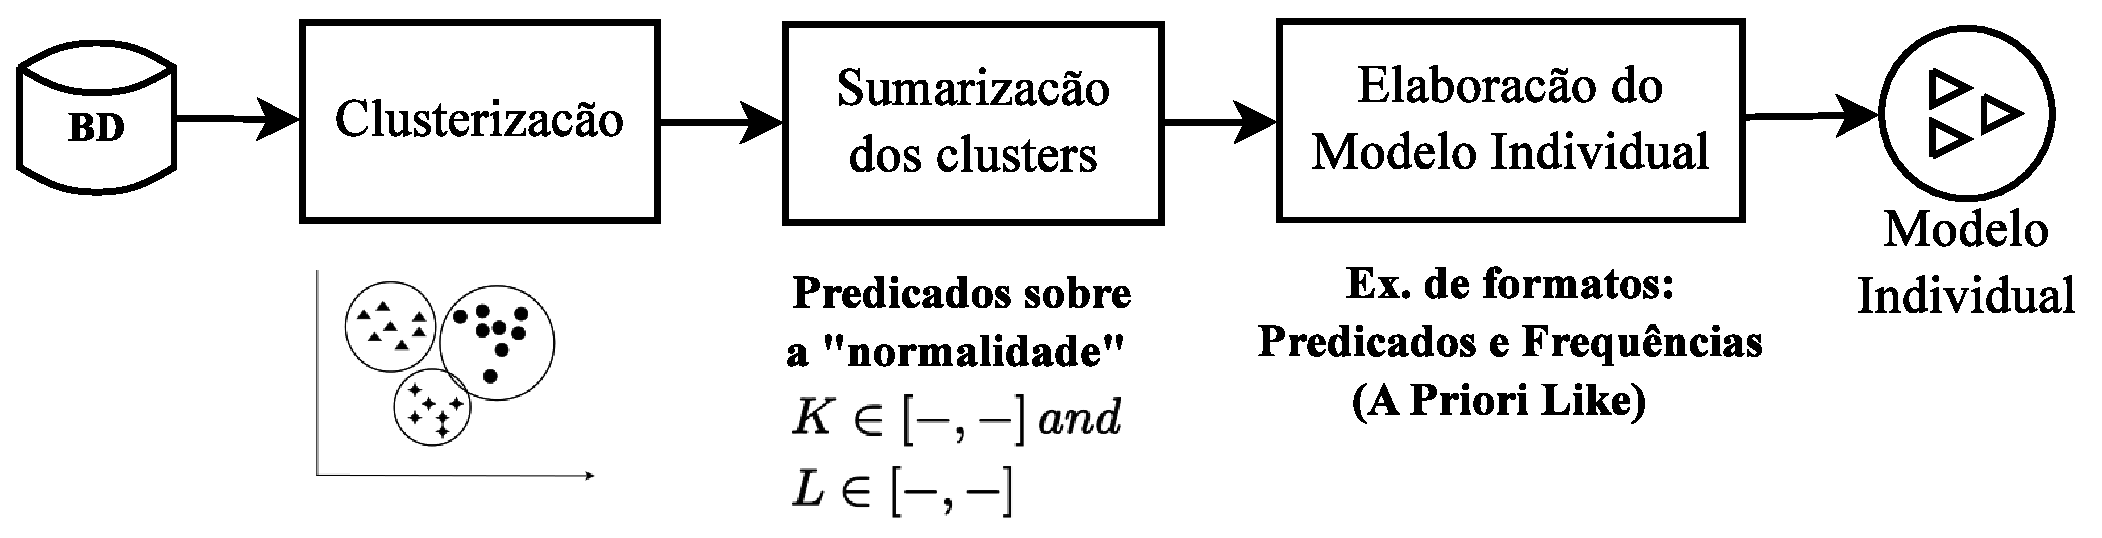
\includegraphics[scale=0.30]{img/VisaoGeral-01}
  		\caption{\scriptsize{Detalhamento da Geração dos Modelos Individuais}}
   	\end{figure}
\end{frame}

\begin{frame}
	\frametitle{Visão Geral -- Módulo Central}
    \begin{figure}
		\centering
	    \includegraphics[scale=0.30]{img/VisaoGeral-02}
  		\caption{\scriptsize{Envio dos modelos para o Módulo Central}}
   	\end{figure}
\end{frame}

\begin{frame}
	\frametitle{Visão Geral -- Módulo Central}
    \begin{figure}
		\centering
	    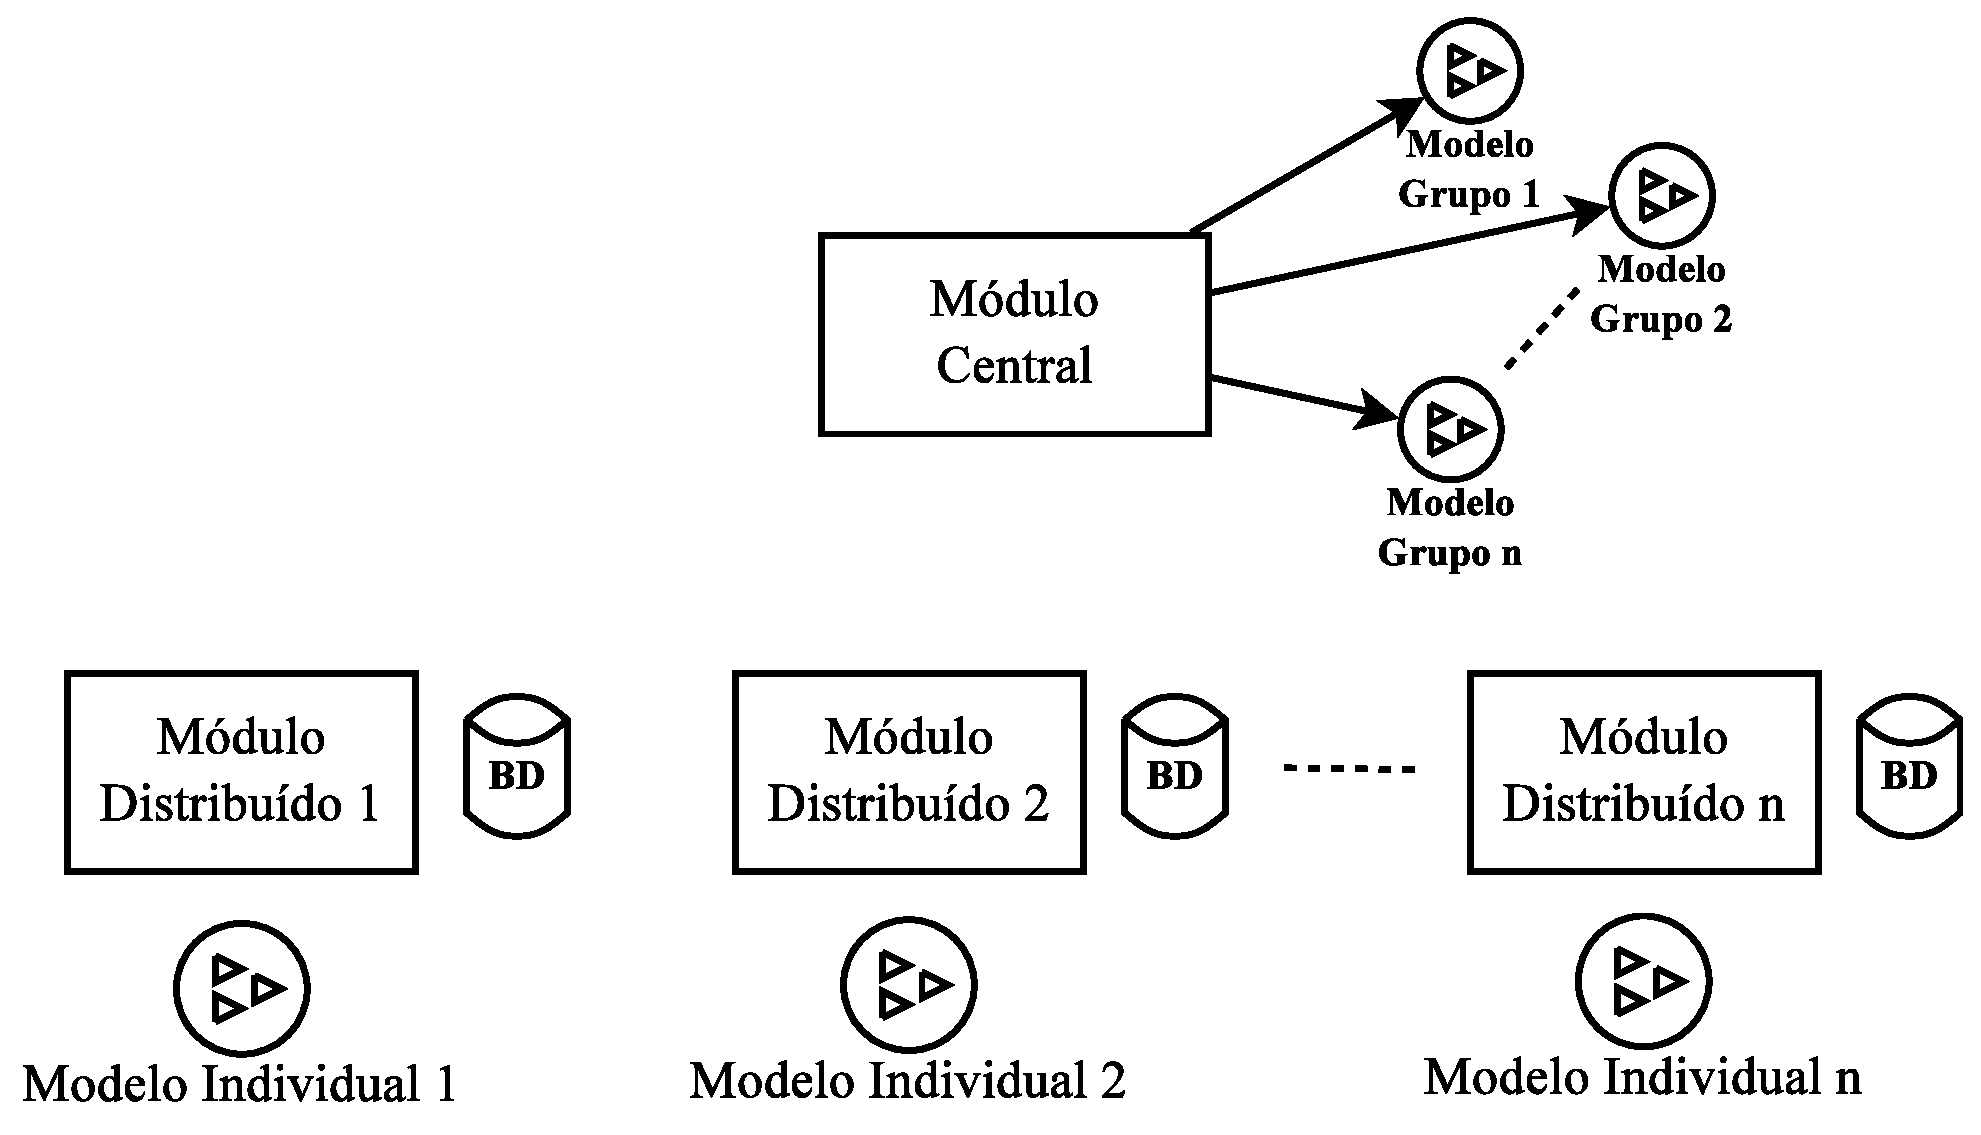
\includegraphics[scale=0.30]{img/VisaoGeral-03}
  		\caption{\scriptsize{Geração dos Modelos de Grupo}}
   	\end{figure}
\end{frame}

\begin{frame}
	\frametitle{Visão Geral -- Geração dos Modelos}
    \begin{figure}
		\centering
	    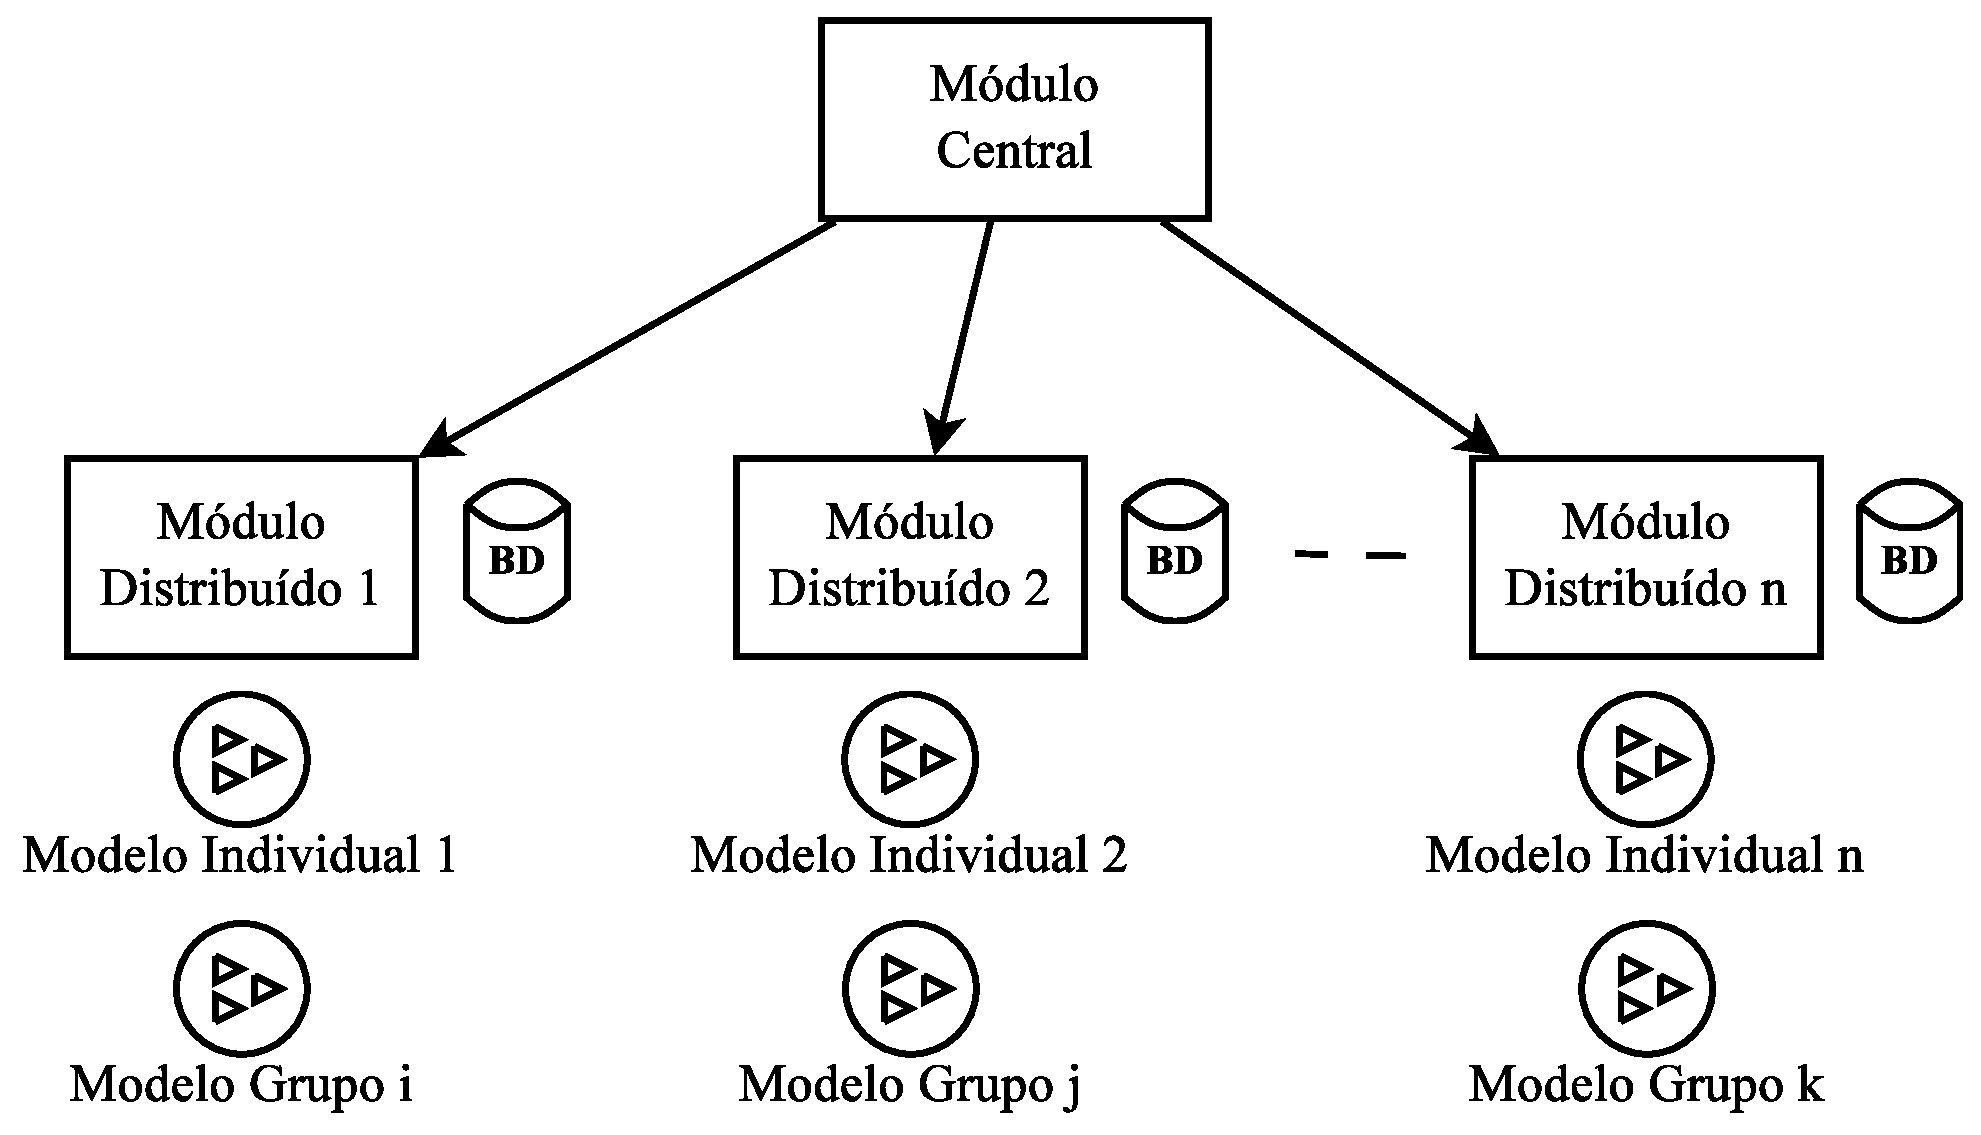
\includegraphics[scale=0.30]{img/VisaoGeral-04}
  		\caption{\scriptsize{Devolução para os Módulos Distribuídos}}
   	\end{figure}
\end{frame}

\begin{frame}
	\frametitle{Visão Geral -- Identificação de Desvios}
    \begin{figure}
		\centering
	    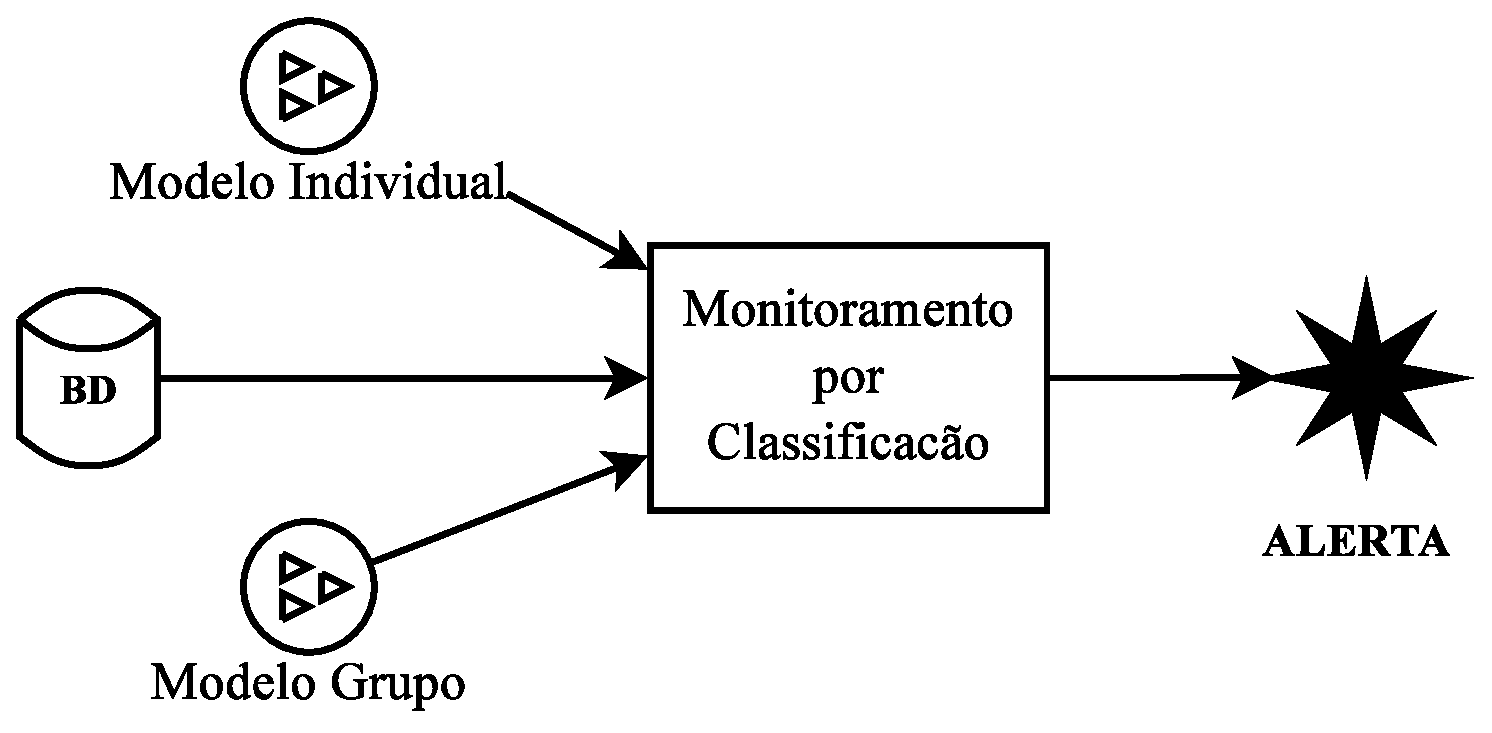
\includegraphics[scale=0.30]{img/VisaoGeral-05}
  		\caption{\scriptsize{Processo de Monitoramento - Mineração Distribuída}}
   	\end{figure}
\end{frame}

\begin{frame}
	\frametitle{Visão Geral -- Identificação de Desvios}
    \begin{figure}
		\centering
	    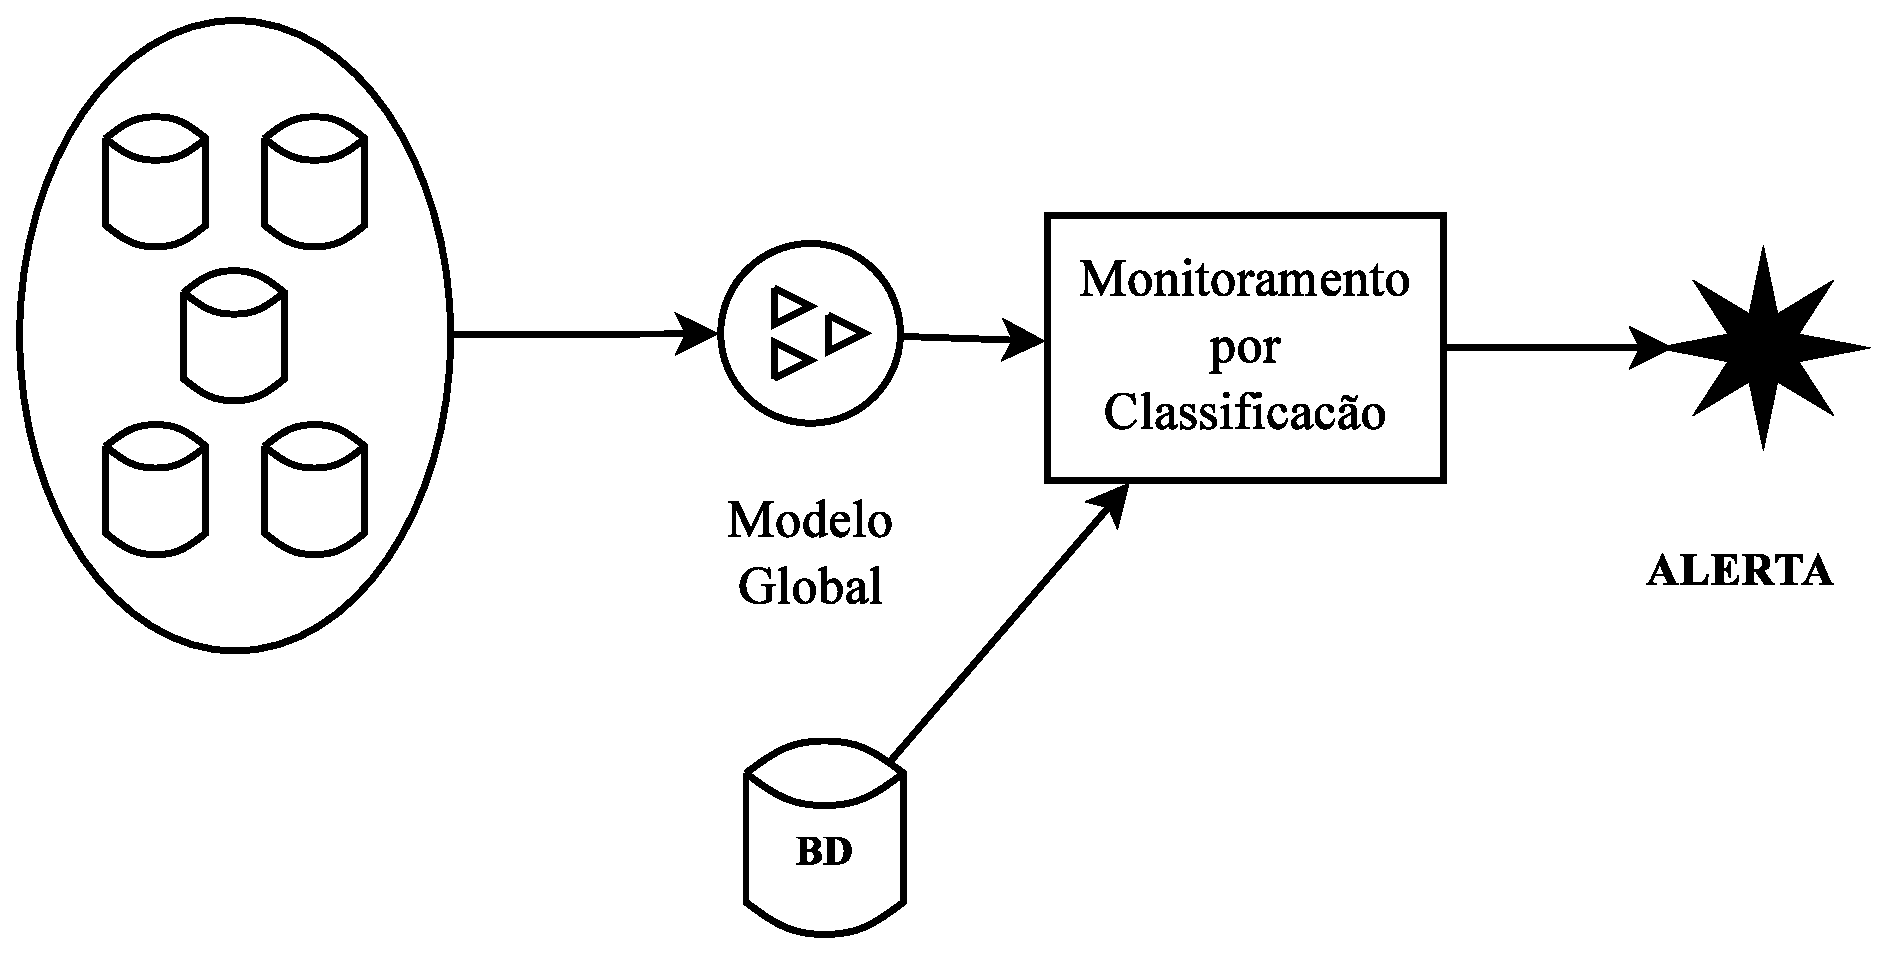
\includegraphics[scale=0.30]{img/VisaoGeral-06}
  		\caption{\scriptsize{Processo de Monitoramento - Mineração Centralizada}}
   	\end{figure}
\end{frame}


\begin{frame}
	\frametitle{Visão Geral}
    Avaliação Mineração Centralizada x Distribuída: \begin{itemize}
	    \item Mensuração a partir da classficação \begin{itemize}
	  	  \item Precisão
          \item F1
	    \end{itemize} 
        \item Volume de dados não transferidos para o nó central
	\end{itemize}
    
\end{frame}
       
\subsection{Viabilidade}  

\begin{frame}
	\frametitle{Viabilidade}
    
    \Large{Ferramentas}
    \normalsize
    \begin{itemize}
   		\item C/C++
		\item Python
        \item Bibliotecas 
    \end{itemize}
    \Large{Datasets}
    \normalsize
    \begin{itemize}
     	\item Produtos de coleta de dados de comportamento \begin{itemize}
        	\item Pulseira (fitBit)
        	\item Telemetria (MyMile)
        \end{itemize}
        \item Análise de clima \begin{itemize}
        	\item Dados públicos
            \item Dados de satélite
        \end{itemize}
    \end{itemize}
    % Dizer como vai fazer. 
    % Falar dos datasets 
    % Citar 
   
\end{frame}

\section{Plano de Ação}

\subsection{Atividades}
\begin{frame}
	\frametitle{Atividades}
    
    \begin{itemize}
	    \item Revisão da Literatura
        \item Identificação de Trabalhos Relacionados
        \item Aprofundamento dos Conceitos Básicos
        \item Detalhamento da Solução Proposta
        \item Implementação do Protótipo
        \item Execução dos Estudos de Caso
        \item Validação e Análise dos Resultados
        \item Produção do Artigo
        \item Escrita da Dissertação
    \end{itemize}
\end{frame}

\subsection{Cronograma}
\begin{frame}
	\frametitle{Cronograma}
		    \begin{figure}
 		   		\centering
	        	\includegraphics[scale=.6]{img/CronogramaDissertacao.png}
   			\end{figure}
 
\end{frame}

\section {Referências}
\begin{frame}[allowframebreaks]
\frametitle{Bibliografia}
    \bibliographystyle{apalike}
    \footnotesize{ \bibliography{ref} }
\end{frame}

\end{document}

